\chapter{Introduction}

\section{Éléments structuraux}
Afin de décrire les différents éléments, on va baser nos hypothèses 
simplificatrices sur une cinématique (déplacement) simplifiée et 
liées aux caractéristiques géométriques. On classera ensuite les 
différentes structures en : 
\begin{itemize}
\item[$\bullet$] \textit{Solides 3D}\\
Il n'existe pas de simplifications "directe", si les dimensions de 
l'objet sont similaires dans les trois directions. Les suivants 
$\bullet$ possèdent des simplifications car une dimension, appelée 
\textbf{épaisseur} est plus petite que les autres.

\item[$\bullet$] \textit{Plaques et coques} (minces ou épaisses)\\
Si la structure est \textbf{plane}, on aura la subdivision suivante 
	\begin{itemize}
	\item Si les efforts sont tous \underline{dans} le plan : \textbf{
	membrane} ; si l'on a de la \textit{tension}.
	\item Si les efforts sont tous \underline{hors} plan  : \textbf{
	plaque} ; si l'on a \textit{flexion} et \textit{cisaillement}
	\item Si les efforts dans le plan \underline{et} hors plan : \textbf{
	coque plane} ; si l'on a \textit{tension, flexion} et \textit{
	cisaillement}
	\end{itemize}
On remarque que dès qu'il y a flexion, il y a cisaillement et si 
en plus on rajoute de la flexion on a une coque plane, par exemple 
une voile.

\item[$\bullet$] \textit{Membranes} (états plans, état axisymétrique)
Si la structure est \textbf{courbe}, on aura la subdivision suivante 
	\begin{itemize}
	\item \textbf{Membrane}
	\item \textbf{Coque}
	\end{itemize}
\begin{center}
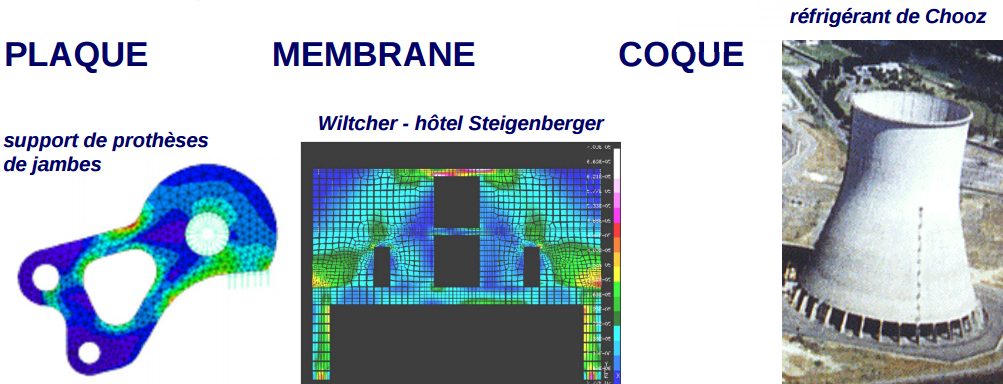
\includegraphics[scale=0.4]{ch1/image1}
\captionof{figure}{Exemples}
\end{center}
\newpage
\item[$\bullet$] \textit{Poutres, arcs} (minces ou épais), \textit{
barres et câbles}\\
Si la structure est \textbf{rectiligne} :
	\begin{itemize}
	\item Si il existe des efforts \underline{hors} axe : 
	\textbf{poutre} ;  si l'on a un effort \textit{normal}, de 
	\textit{flexion} et de \textit{cisaillement}
	\item Si les efforts sont uniquement \underline{selon} axe : 
	\textbf{barre}	;  si l'on a un effort de \textit{compression} 
	et de \textit{traction}
	\item \textbf{cable}	;  si l'on a un effort uniquement dans l'axe 
	sans résistance à la compression ; \textit{traction}
	\end{itemize}
Si la structure est \textbf{courbe} :
	\begin{itemize}
	\item \textbf{Arc } : \textit{flexion + tension + cisaillement}
	\end{itemize}	
	
\begin{center}
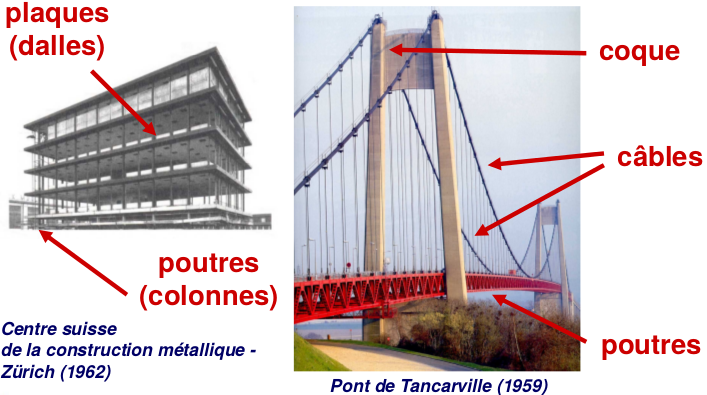
\includegraphics[scale=0.5]{ch1/image2}
\captionof{figure}{Exemples}
\end{center}
\end{itemize}



\section{Principe de Barré de Saint-Venant}
Si l'on considère une section \textbf{éloignée} des points d'application 
des forces, les contraintes ne sont fonction que de la résultante et du 
moment résultant du systèmes de ces forces.\\
La conséquence - que l'on appliquera toujours - est la suivante :\\

\retenir{Si on ne s'intéresse pas à la zone proche\footnote{A moins de deux 
fois la plus grande dimension transversale.} des forces, on peut 
remplacer celles-ci par leur résultante et leurs moments résultants}